\documentclass[
a5paper,
10pt, 
onecolumn,
openany,
]{memoir}

\usepackage{fontspec}
\usepackage[raggedright,bf,sf]{titlesec}
\usepackage{titletoc}
\usepackage{titling}
\usepackage{nameref}
\usepackage[german]{babel} % English please
\usepackage[final]{microtype} % Less badboxes
\usepackage{graphicx} % Include figures
\usepackage{lipsum} % Just to put in some text
\usepackage{xcolor}
\usepackage{caption}

%\usepackage{merriweather}
%\usepackage{librecaslon} % Caslon font

\setmainfont{Recia}
%\setsansfont{Author}
%\setsansfont{Switzer} %zu modern
\setsansfont{Myriad Pro}
%\setsansfont{Merriweather Sans}

\renewcommand{\printtoctitle}[1]{\LARGE\sffamily\bfseries #1}
\renewcommand{\cftchapterfont}{\sffamily\bfseries}
\renewcommand{\cftchapterpagefont}{\sffamily\bfseries}
\renewcommand{\cftsectionfont}{\sffamily}
\renewcommand{\cftsectionpagefont}{\sffamily}
\renewcommand{\cftsubsectionfont}{\sffamily}
\renewcommand{\cftsubsectionpagefont}{\sffamily}
\renewcommand{\cftsubsubsectionfont}{\sffamily}
\renewcommand{\cftsubsubsectionpagefont}{\sffamily}
\renewcommand{\printloftitle}[1]{\LARGE\sffamily #1}
\renewcommand{\cftfigurefont}{\sffamily}
\renewcommand{\cftfigurepagefont}{\sffamily}
\renewcommand{\printlottitle}[1]{\LARGE\sffamily #1}
\renewcommand{\cfttablefont}{\sffamily}
\renewcommand{\cfttablepagefont}{\sffamily}

\newcommand{\tabref}[1]{Tabelle \ref{#1}: \nameref{#1}}

\captionsetup{%
  font={normalsize}, % small font size
  labelfont={it},      % label in bold, sans-serif
  textfont={it},
  singlelinecheck=true, % centered single-lined captions
  format=plain,             % indention=1cm,
  labelsep={colon},         % default separator: none, colon, period, space, quad, newline, endash
}

\titleformat{\chapter}[display]{\sffamily\bfseries\LARGE}{\raggedleft\HUGE\textcolor{gray}{\normalfont\thechapter}}{0.5em}{}[\titlerule]
\titleformat*{\section}{\sffamily\LARGE}
\titleformat*{\subsection}{\sffamily\Large}
\titleformat*{\subsubsection}{\sffamily\large}
\titleformat*{\paragraph}{\sffamily\large}
\titleformat*{\subparagraph}{\sffamily\large}

\setlrmarginsandblock{0.15\paperwidth}{*}{1} % Left and right margin
\setulmarginsandblock{0.2\paperwidth}{*}{1}  % Upper and lower margin
\checkandfixthelayout

\maxsecnumdepth{subsection} % Subsections (and higher) are numbered
\setsecnumdepth{subsection}

\chapterstyle{standard}

\makeatletter                  % You do not need to write [htpb] all the time
\renewcommand\fps@figure{htbp} %
\renewcommand\fps@table{htbp}  %
\makeatother                   %

%%% HEADER AND FOOTER 
%%%------------------------------------------------------------------------------

\makepagestyle{standard} % Make standard pagestyle

\makeatletter                 % Define standard pagestyle
\makeevenfoot{standard}{\small\sffamily\thepage}{}{} %
\makeoddfoot{standard}{}{}{\small\sffamily\thepage}  %
\makeevenhead{standard}{\textcolor{gray}{\sffamily\small\leftmark}}{}{}
\makeoddhead{standard}{}{}{\textcolor{gray}{\sffamily\small\rightmark}}
\makeheadrule{standard}{\textwidth}{\normalrulethickness}
\makeatother                  %

\makeatletter
\makepsmarks{standard}{
\createmark{chapter}{both}{shownumber}{}{ \quad }
\createmark{section}{right}{shownumber}{}{ \quad }
\createplainmark{toc}{both}{\contentsname}
\createplainmark{lof}{both}{\listfigurename}
\createplainmark{lot}{both}{\listtablename}
\createplainmark{bib}{both}{\bibname}
\createplainmark{index}{both}{\indexname}
\createplainmark{glossary}{both}{\glossaryname}
}
\makeatother                               %

\makepagestyle{chap} % Make new chapter pagestyle

\makeatletter
\makeevenfoot{chap}{\small\sffamily\thepage}{}{} % Define new chapter pagestyle
\makeoddfoot{chap}{}{}{\small\sffamily\thepage}  %
\makeevenhead{chap}{}{}{}   %
\makeoddhead{chap}{}{}{}    %
%\makeheadrule{chap}{\textwidth}{\normalrulethickness}
\makeatother

\nouppercaseheads
\pagestyle{standard}               % Choosing pagestyle and chapter pagestyle
\aliaspagestyle{chapter}{chap} %

\maxtocdepth{subsection} % Only parts, chapters and sections in the table of contents
\settocdepth{subsection}

\author{}
\title{\sffamily\Huge Chronik zum 200-jährigen Bestehen der Schützenbruderschaft St. Hubertus Niederense 1824 e.V.}
\date{\sffamily Herausgegeben im Juli 2024}

\begin{document}

\raggedbottom

\frontmatter

\maketitle

%\thispagestyle{empty}
\begingroup
\footnotesize
\parindent 0pt
\parskip \baselineskip
\textcopyright{} 2024 Schützenbruderschaft St. Hubertus Niederense 1824 e.V.

Alle Rechte vorbehalten.

\lipsum[1-1]

% \begin{center}
%  99 32 11 88 48 01\hspace{2em}9 9 8 6 5 4 %1 
% \end{center}

\vfill

Erstausgabe: Juli 2024

Autoren: \\
\hspace*{2em} Tobias Bäcker, Lars Bittis, Roland Gerasch \\
\hspace*{2em} Ludwig Brinkmann, Ewald Wulff \\
\\
Satz und Gestaltung: \\
\hspace*{2em} Tobias Bäcker, Tobias Schulte \\
\\
\\
Herausgeber: \\
\\
\hspace*{2em} Schützenbruderschaft St. Hubertus Niederense 1824 e.V. \\
\hspace*{2em} Heuerwerth 5 \\
\hspace*{2em} 59469 Ense \\
\\
\hspace*{2em} info@schuetzen-niederense.de

\endgroup
\clearpage

\cleartooddpage

\tableofcontents*

\cleartooddpage

\chapter{Vorwort}

Dies ist ein Typoblindtext. An ihm kann man sehen, ob alle Buchstaben da sind und wie sie aussehen. Manchmal benutzt man Worte wie Hamburgefonts, Rafgenduks oder Handgloves, um Schriften zu testen. Manchmal Sätze, die alle Buchstaben des Alphabets enthalten - man nennt diese Sätze »Pangrams«. Sehr bekannt ist dieser: The quick brown fox jumps over the lazy old dog. Oft werden in Typoblindtexte auch fremdsprachige Satzteile eingebaut (AVAIL® and Wefox™ are testing aussi la Kerning), um die Wirkung in anderen Sprachen zu testen. In Lateinisch sieht zum Beispiel fast jede Schrift gut aus. Quod erat demonstrandum. Seit 1975 fehlen in den meisten Testtexten die Zahlen, weswegen nach TypoGb. 204 § ab dem Jahr 2034 Zahlen in 86 der Texte zur Pflicht werden. Nichteinhaltung wird mit bis zu 245 € oder 368 \$ bestraft. Genauso wichtig in sind mittlerweile auch Âçcèñtë, die in neueren Schriften aber fast immer enthalten sind. Ein wichtiges aber schwierig zu integrierendes Feld sind OpenType-Funktionalitäten. Je nach Software und Voreinstellungen können eingebaute Kapitälchen, Kerning oder Ligaturen (sehr pfiffig) nicht richtig dargestellt werden.

\begin{figure}
  \centering
  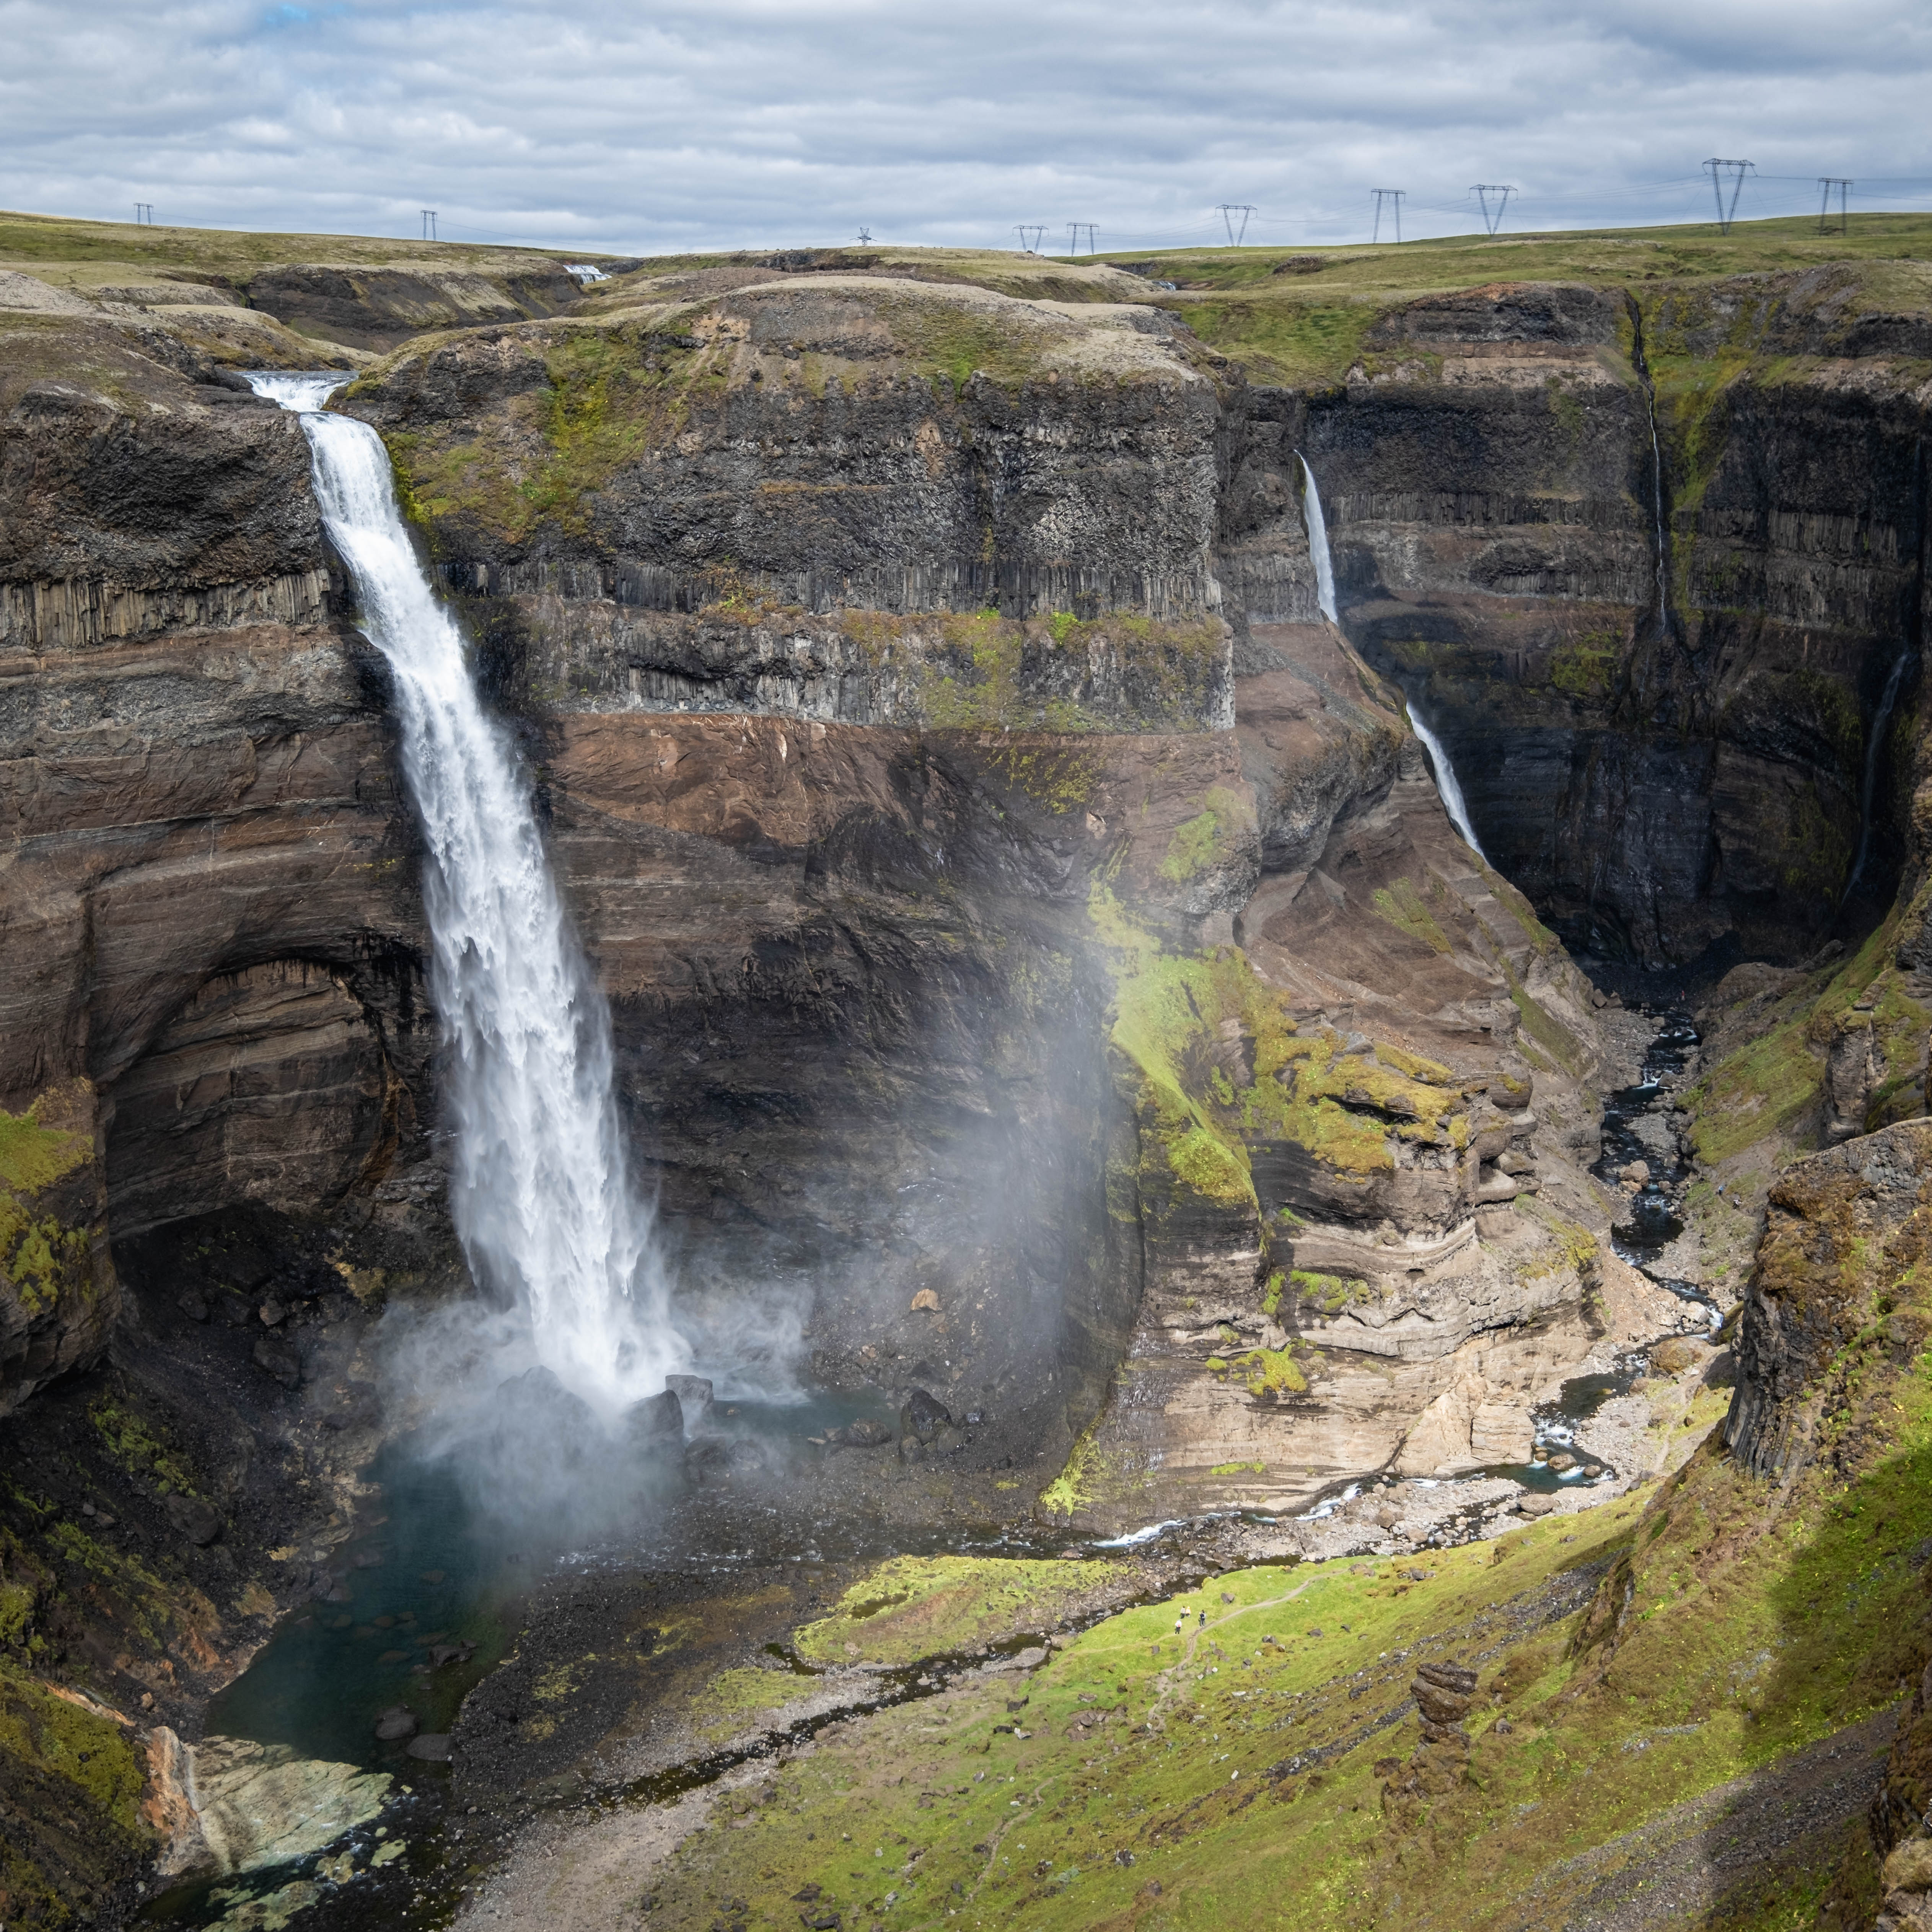
\includegraphics[width=0.9\textwidth]{fotos/a}
  \caption{Ein Bär}
\end{figure}

Manchmal benutzt man Worte wie Hamburgefonts, Rafgenduks oder Handgloves, um Schriften zu testen. Manchmal Sätze, die alle Buchstaben des Alphabets enthalten - man nennt diese Sätze »Pangrams«. Sehr bekannt ist dieser: The quick brown fox jumps over the lazy old dog. Oft werden in Typoblindtexte auch fremdsprachige Satzteile eingebaut (AVAIL® and Wefox™ are testing aussi la Kerning), um die Wirkung in anderen Sprachen zu testen. In Lateinisch sieht zum Beispiel fast jede Schrift gut aus. Quod erat demonstrandum. Seit 1975 fehlen in den meisten Testtexten die Zahlen, weswegen nach TypoGb. 204 § ab dem Jahr 2034 Zahlen in 86 der Texte zur Pflicht werden. Nichteinhaltung wird mit bis zu 245 € oder 368 \$ bestraft. Genauso wichtig in sind mittlerweile auch Âçcèñtë, die in neueren Schriften aber fast immer enthalten sind. Ein wichtiges aber schwierig zu integrierendes Feld sind OpenType-Funktionalitäten. Je nach Software und Voreinstellungen können eingebaute Kapitälchen, Kerning oder Ligaturen (sehr pfiffig) nicht richtig dargestellt werden.

An ihm kann man sehen, ob alle Buchstaben da sind und wie sie aussehen. Manchmal benutzt man Worte wie Hamburgefonts, Rafgenduks oder Handgloves, um Schriften zu testen. Manchmal Sätze, die alle Buchstaben des Alphabets enthalten - man nennt diese Sätze »Pangrams«. Sehr bekannt ist dieser: The quick brown fox jumps over the lazy old dog. Oft werden in Typoblindtexte auch fremdsprachige Satzteile eingebaut (AVAIL® and Wefox™ are testing aussi la Kerning), um die Wirkung in anderen Sprachen zu testen. In Lateinisch sieht zum Beispiel fast jede Schrift gut aus. Quod erat demonstrandum. Seit 1975 fehlen in den meisten Testtexten die Zahlen, weswegen nach TypoGb. 204 § ab dem Jahr 2034 Zahlen in 86 der Texte zur Pflicht werden. Nichteinhaltung wird mit bis zu 245 € oder 368 \$ bestraft. Genauso wichtig in sind mittlerweile auch Âçcèñtë, die in neueren Schriften aber fast immer enthalten sind. Ein wichtiges aber schwierig zu integrierendes Feld sind OpenType-Funktionalitäten. Je nach Software und Voreinstellungen können eingebaute Kapitälchen, Kerning oder Ligaturen (sehr pfiffig) nicht richtig dargestellt werden.

\mainmatter

\chapter{Wie man eine Zeitmaschine baut}

\lipsum[1-1] 

\section{Anforderungen}

\lipsum[1-1]

\begin{table}
  \centering
  \begin{tabularx}{0.9\textwidth}{ c l l X }
    Jahr & Name & Partner & \\
    \hline\noalign{\smallskip}
    1906 & Peter Pan & Petra & toller König \\ 
    1907 & Max Müller & Mimi &  \\  
    1908 & Susi Sommer & Simon & erste Frau \\
    1906 & Peter Pan & Petra & toller König \\ 
    1907 & Max Müller & Mimi &  \\  
    1907 & Max Müller & Mimi &  \\  
    1908 & Susi Sommer & Simon & erste Frau \\
    1906 & Peter Pan & Petra & toller König \\ 
    1907 & Max Müller & Mimi &  \\  
    1908 & Susi Sommer & Simon & erste Frau \\
  \end{tabularx}
  \caption{Könige historisch}
  \label{fig:tab_koenige_historisch}
\end{table}

\section{Ausführung}

\lipsum[1-1]

\begin{figure}
  \centering
  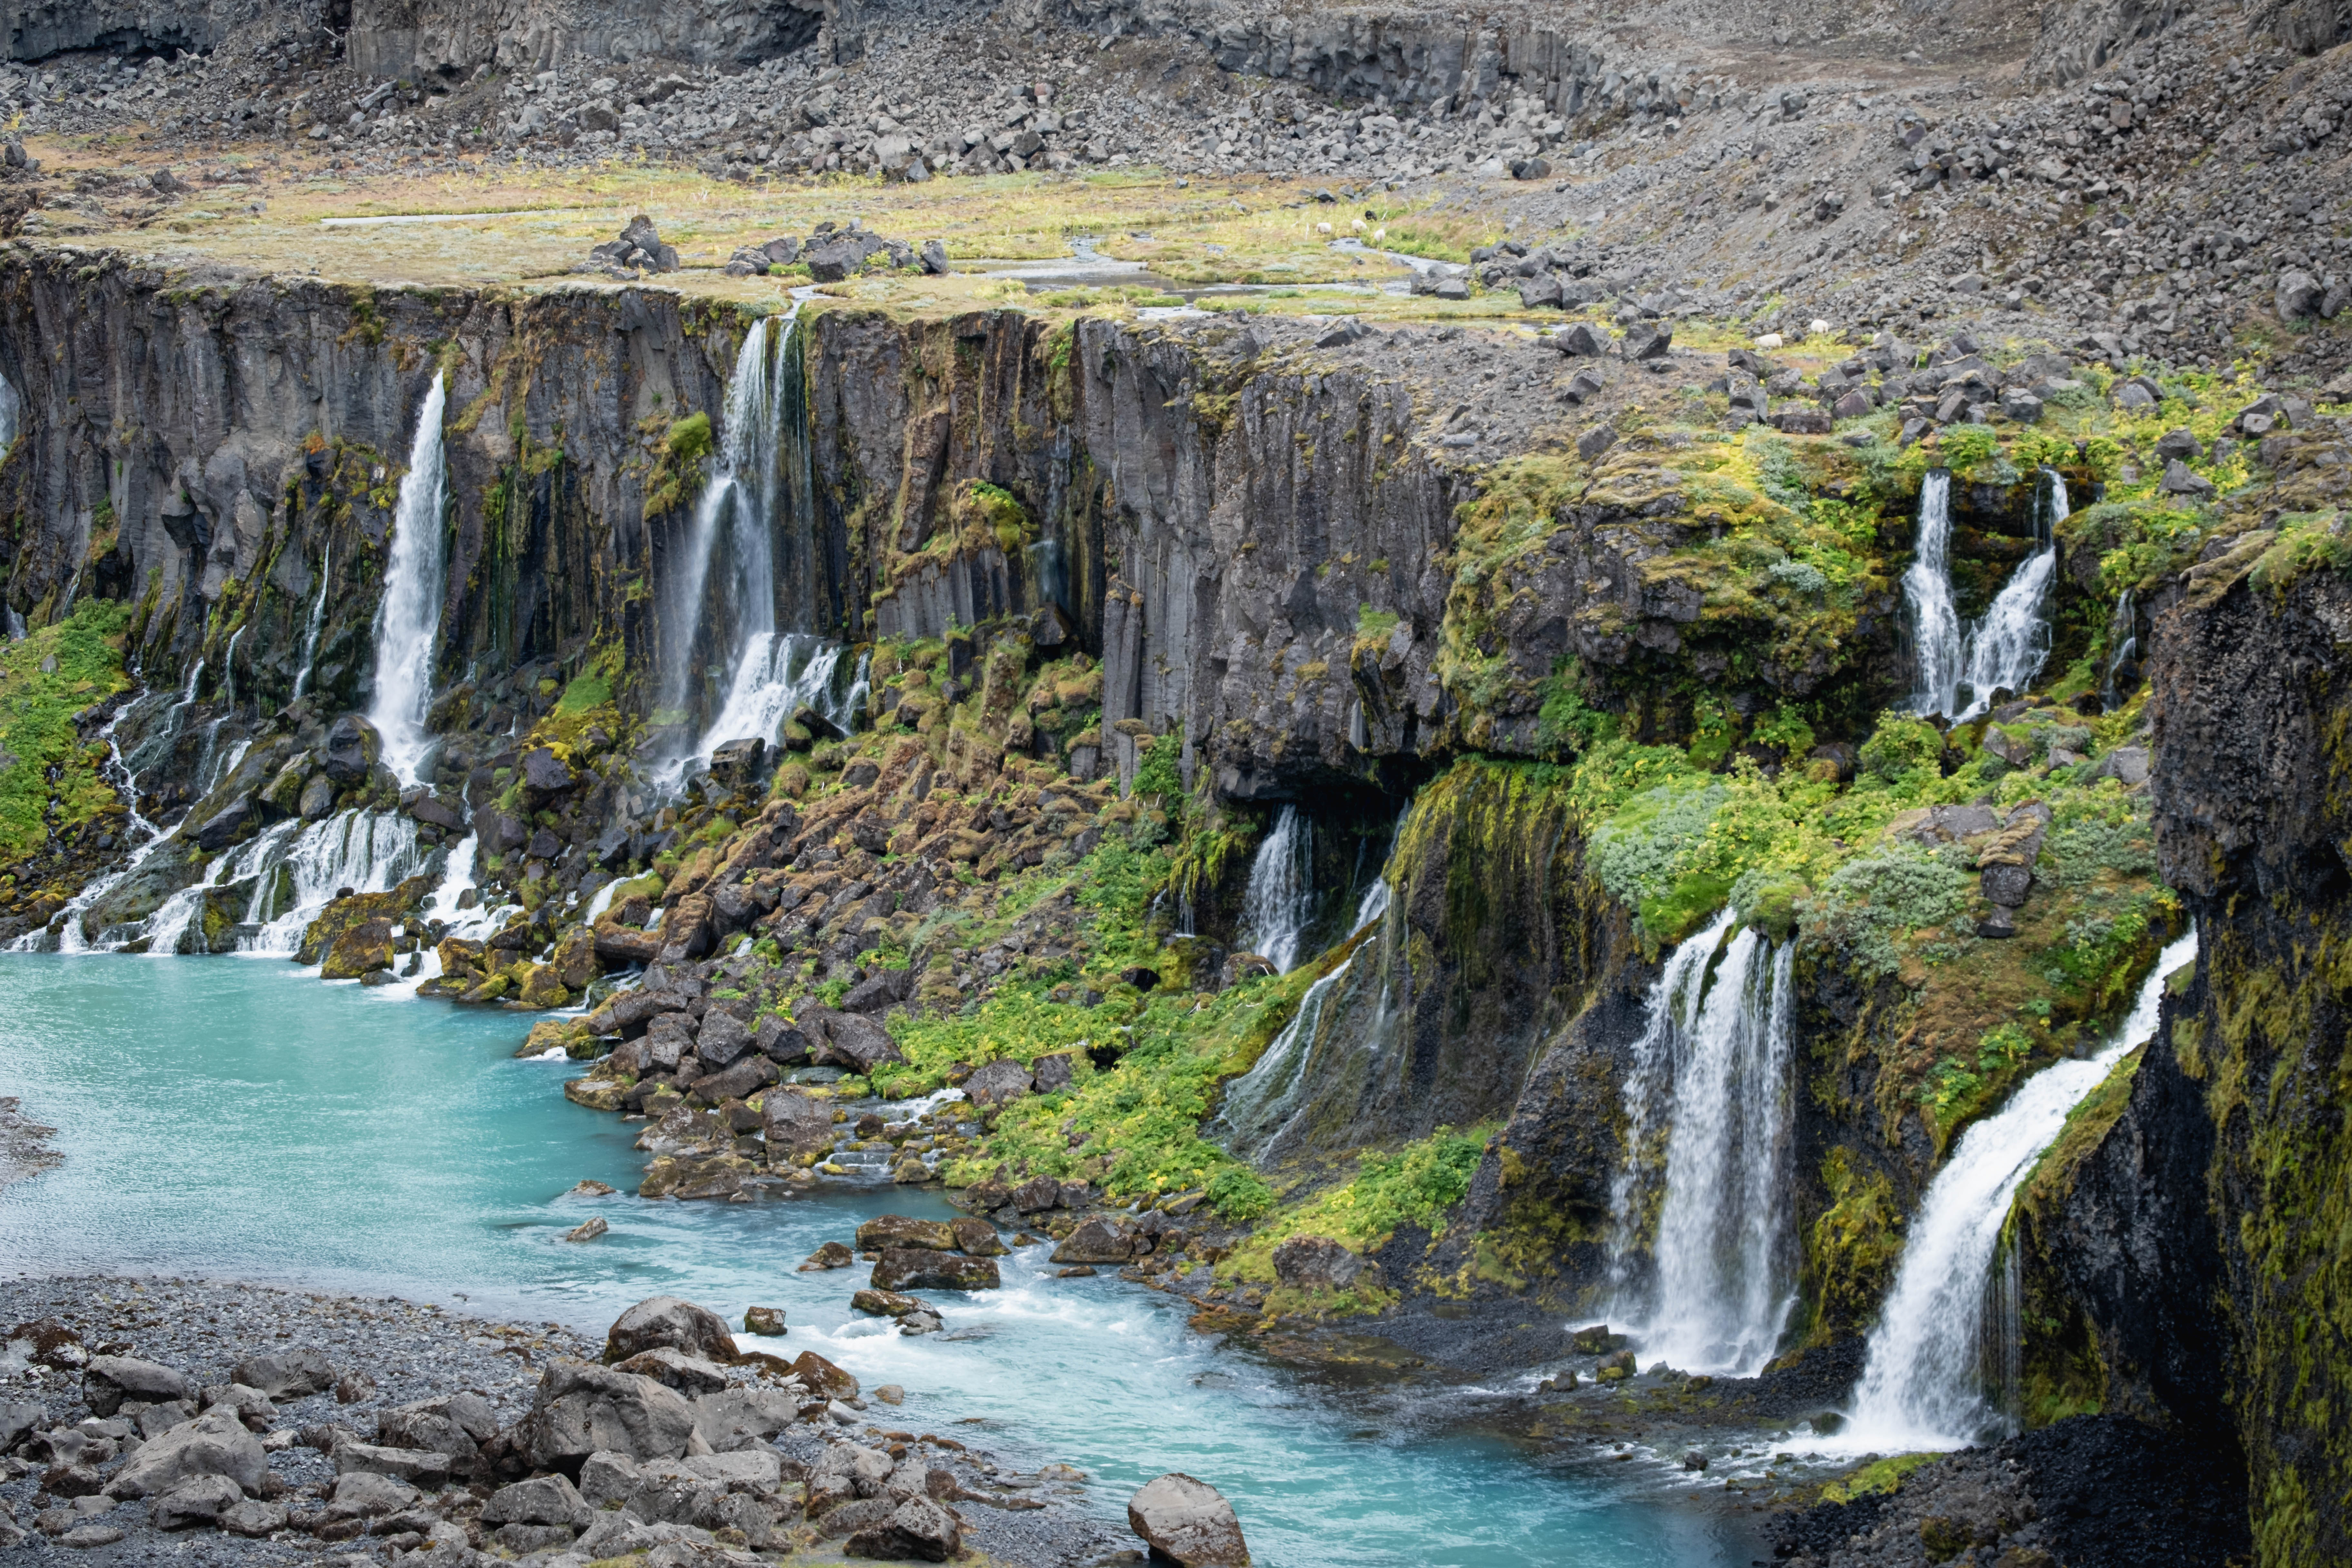
\includegraphics[width=0.3\textwidth]{fotos/b}
  \caption{Noch ein Bär}
\end{figure}

\lipsum[1-4]

\chapter{Wie man eine Zeitmaschine zerstört}

\lipsum[1-3]

\section{Ausrüstung}

Jemand musste Josef K. verleumdet haben, denn ohne dass er etwas Böses getan hätte, wurde er eines Morgens verhaftet. »Wie ein Hund! « sagte er, es war, als sollte die Scham ihn überleben. Als Gregor Samsa eines Morgens aus unruhigen Träumen erwachte, fand er sich in seinem Bett zu einem ungeheueren Ungeziefer verwandelt.

Und es war ihnen wie eine Bestätigung ihrer neuen Träume und guten Absichten, als am Ziele ihrer Fahrt die Tochter als erste sich erhob und ihren jungen Körper dehnte. »Es ist ein eigentümlicher Apparat«, sagte der Offizier zu dem Forschungsreisenden und überblickte mit einem gewissermaßen bewundernden Blick den ihm doch wohlbekannten Apparat.
%TODO mehr platz?

Sie hätten noch ins Boot springen können, aber der Reisende hob ein schweres, geknotetes Tau vom Boden, drohte ihnen damit und hielt sie dadurch von dem Sprunge ab. In den letzten Jahrzehnten ist das Interesse (siehe \tabref{fig:tolle_tabelle}) an Hungerkünstlern sehr zurückgegangen. Aber sie überwanden sich, umdrängten den Käfig und wollten sich gar nicht fortrühren. Jemand musste Josef K. verleumdet haben, denn ohne dass er etwas Böses getan hätte, wurde er eines Morgens verhaftet. »Wie ein Hund! « sagte er, es war, als sollte die Scham ihn überleben. Als Gregor Samsa eines Morgens aus unruhigen Träumen erwachte, fand er sich

\section{Erfahrung}

\lipsum[1-1]

\section{Testergebnisse}

\lipsum[1-1]

\subsection{Test 1}

Test fehlgeschlagen

\subsection{Test 2}

\begin{table}
\centering
\begin{tabularx}{0.9\textwidth}{l | c X}
abc & asd & gfdf g \\
asjdlasd & as  d & sd546dfg \\
asjda & dfhjsdf & flkhgölf kgh \\
\end{tabularx}
\caption{Testergebnisse}
\label{fig:tolle_tabelle}
\end{table}

\subsection{Schulisch}

\begin{figure}
  \centering
  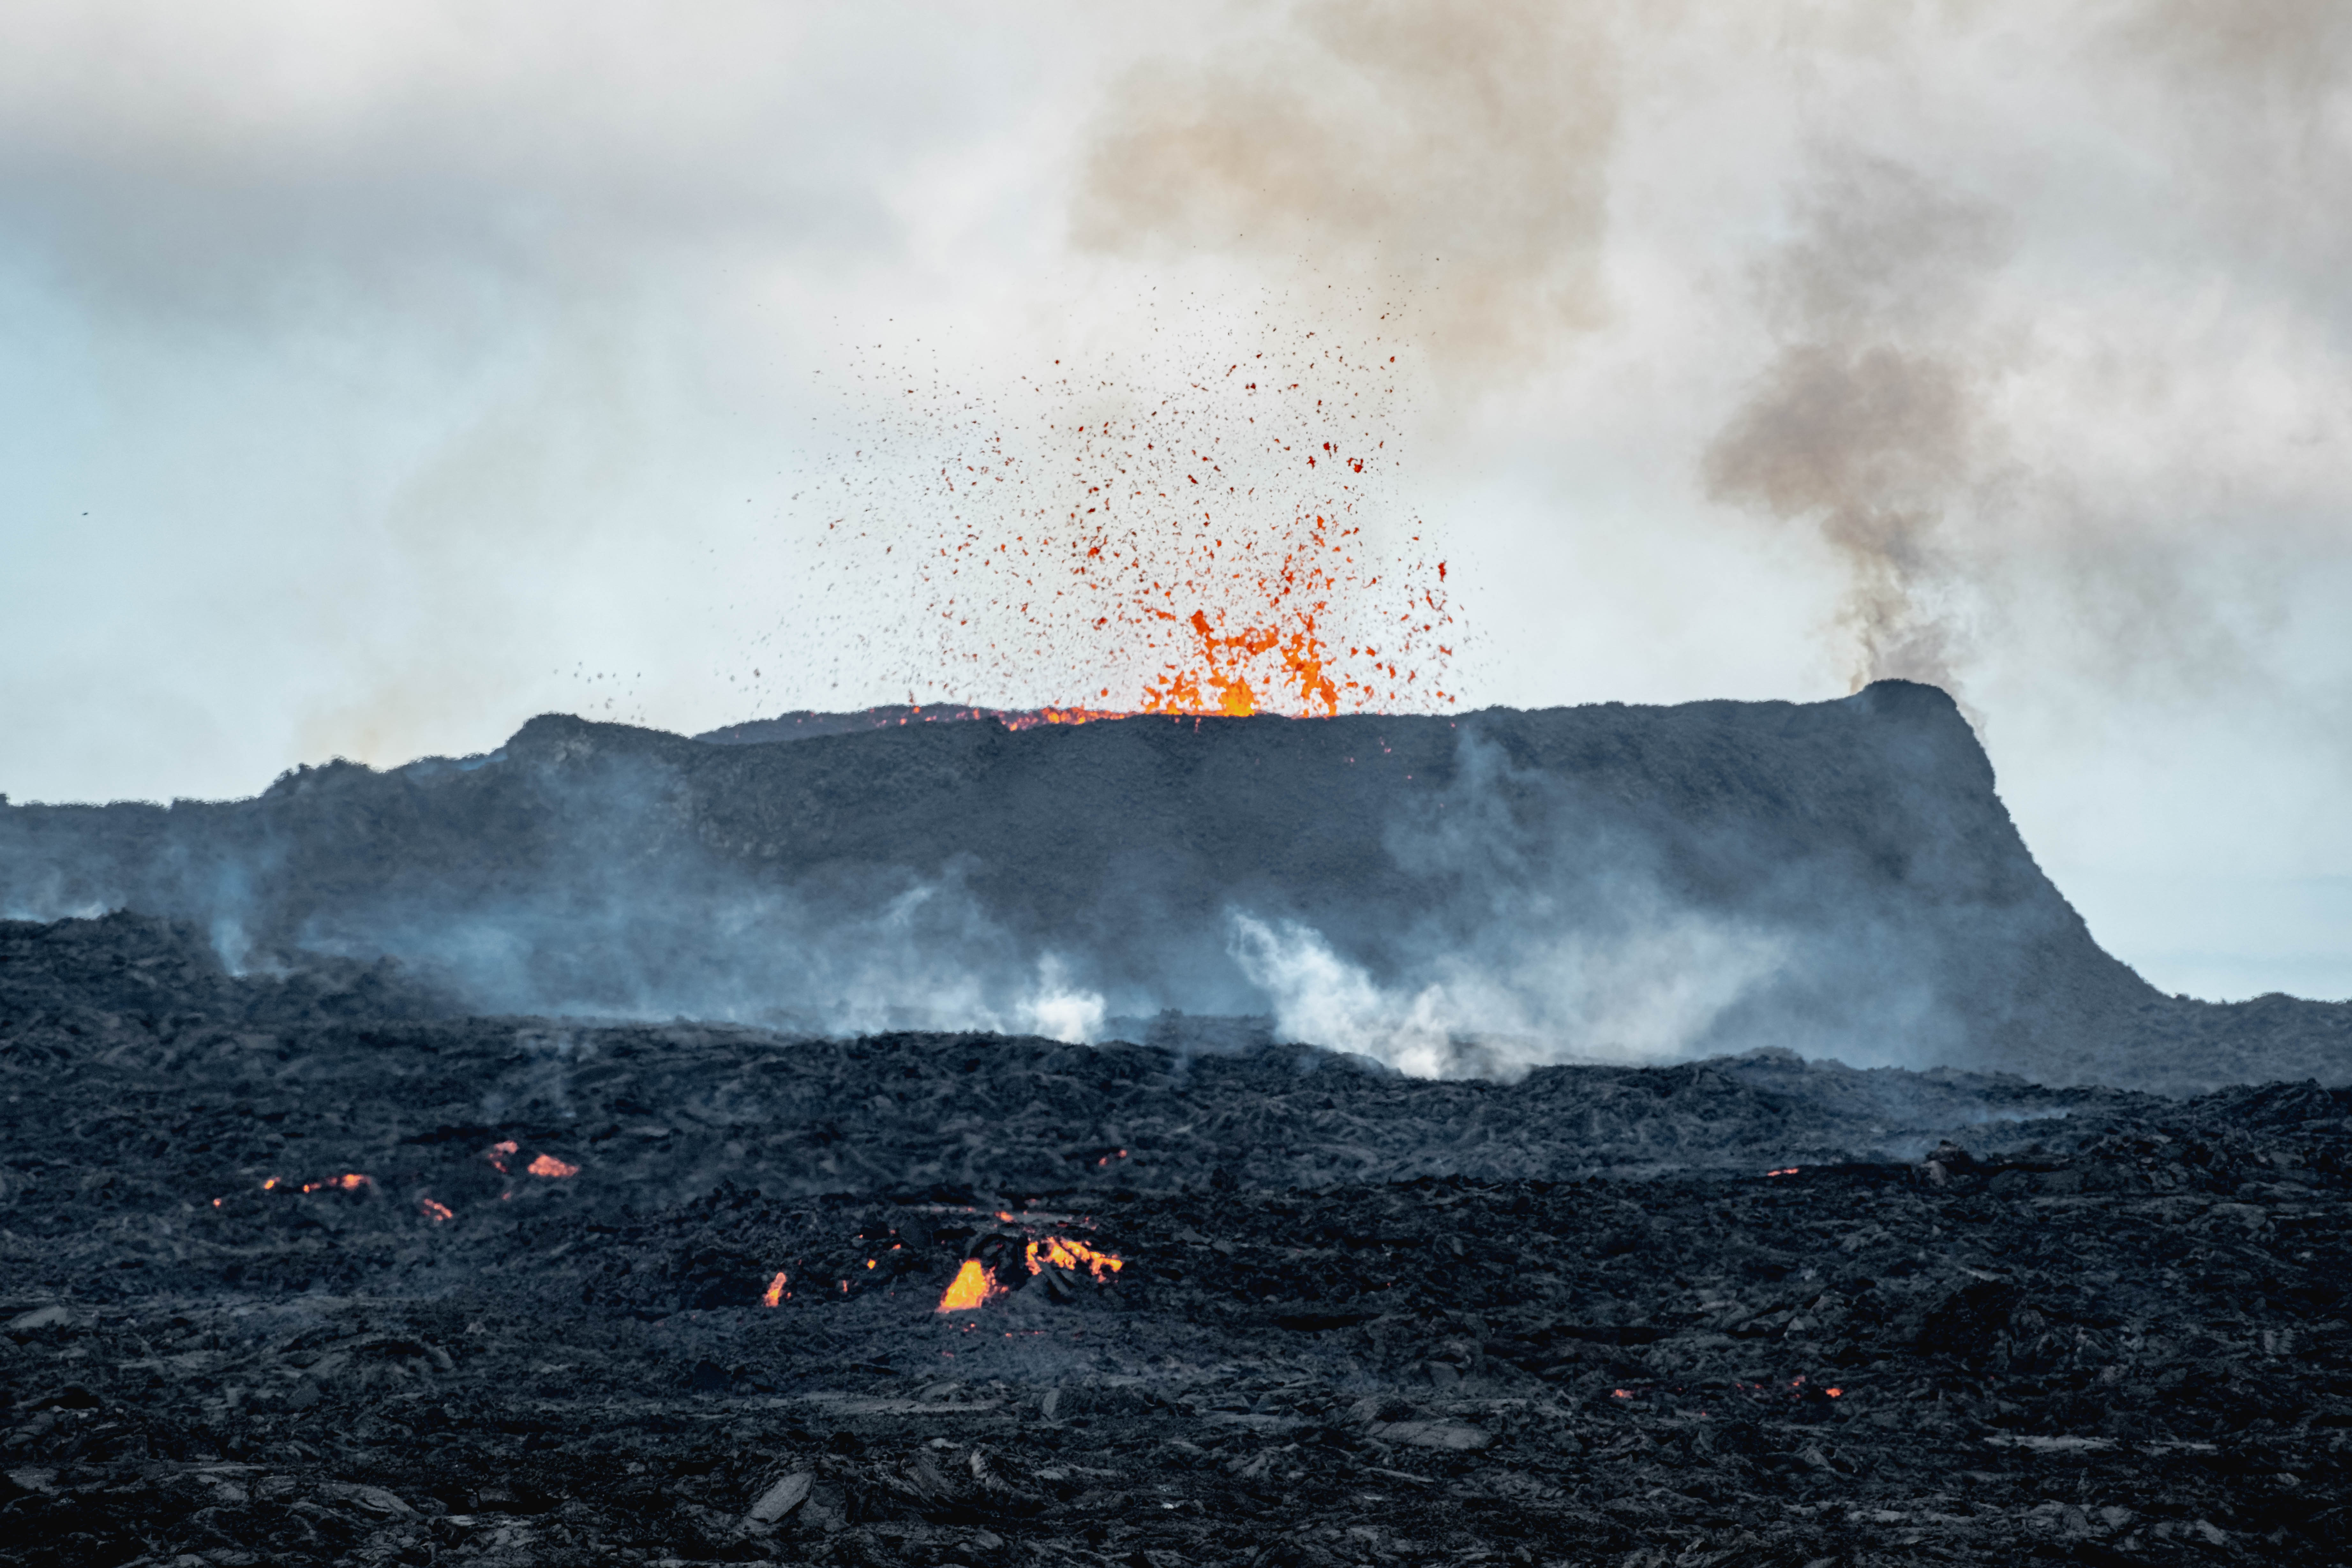
\includegraphics[width=0.8\textwidth]{fotos/d}
  \caption{Mehr Bär}
\end{figure}

\lipsum[1-5]

\subsection{Arbeitsumfeld}

\lipsum[1-2]

\cleartooddpage
 
\thispagestyle{empty}
\listoffigures
\cleartooddpage

\thispagestyle{empty}
\listoftables
\cleartooddpage

\appendix

\chapter{Kausalität}

Dies ist ein Typoblindtext. An ihm kann man sehen, ob alle Buchstaben da sind und wie sie aussehen. Manchmal benutzt man Worte wie Hamburgefonts, Rafgenduks oder Handgloves, um Schriften zu testen. Manchmal Sätze, die alle Buchstaben des Alphabets enthalten - man nennt diese Sätze »Pangrams«. Sehr bekannt ist dieser: The quick brown fox jumps over the lazy old dog. Oft werden in Typoblindtexte auch fremdsprachige Satzteile eingebaut (AVAIL® and Wefox™ are testing aussi la Kerning), um die Wirkung in anderen Sprachen zu testen. In Lateinisch sieht zum Beispiel fast jede Schrift gut aus. Quod erat demonstrandum. Seit 1975 fehlen in den meisten Testtexten die Zahlen, weswegen nach TypoGb. 204 § ab dem Jahr 2034 Zahlen in 86 der Texte zur Pflicht werden. Nichteinhaltung wird mit bis zu 245 € oder 368 \$ bestraft. Genauso wichtig in sind mittlerweile auch Âçcèñtë, die in neueren Schriften aber fast immer enthalten sind. Ein wichtiges aber schwierig zu integrierendes Feld sind OpenType-Funktionalitäten. Je nach Software und Voreinstellungen können eingebaute Kapitälchen, Kerning oder Ligaturen (sehr pfiffig) nicht richtig dargestellt werden.

Manchmal Sätze, die alle Buchstaben des Alphabets enthalten - man nennt diese Sätze »Pangrams«. Sehr bekannt ist dieser: The quick brown fox jumps over the lazy old dog. Oft werden in Typoblindtexte auch fremdsprachige Satzteile eingebaut (AVAIL® and Wefox™ are testing aussi la Kerning), um die Wirkung in anderen Sprachen zu testen. In Lateinisch sieht zum Beispiel fast jede Schrift gut aus. Quod erat demonstrandum. Seit 1975 fehlen in den meisten Testtexten die Zahlen, weswegen nach TypoGb. 204 § ab dem Jahr 2034 Zahlen in 86 der Texte zur Pflicht werden. Nichteinhaltung wird mit bis zu 245 € oder 368 \$ bestraft. Genauso wichtig in sind mittlerweile auch Âçcèñtë, die in neueren Schriften aber fast immer enthalten sind. Ein wichtiges aber schwierig zu integrierendes Feld sind OpenType-Funktionalitäten. Je nach Software und Voreinstellungen können eingebaute Kapitälchen, Kerning oder Ligaturen (sehr pfiffig) nicht richtig dargestellt werden.

\backmatter

\end{document}